\documentclass[10 pt]{article}

\usepackage{fontspec}
\defaultfontfeatures{Mapping=tex-text}
\setmainfont{Minion Pro}

%\usepackage{graphicx}
%\usepackage{fullpage}
\usepackage{pdfpages}
\usepackage{lastpage, fancyhdr}
\pagestyle{fancy}
\lhead{Scott O'Connor}
\chead{Phil 234} 
\rhead{\emph{Overview}}
\lfoot{}
\cfoot{\thepage\space of \pageref{LastPage}} 
\rfoot{}

\thispagestyle{empty}


\begin{document}
\author{Phil 234}
\title{Overview}
\maketitle
\section*{Chronology of Major Historical Events}
\begin{itemize}
\item{c. 12th Century BCE: Trojan War, North Turkey,  semi-mythical, the last year is recounted in Homer's \emph{Iliad}}
\item{8th Century BCE: Greek colonies populate southern Italy, Ionia (western Turkey), and elsewhere, Greek religion described by Hesiod holds sway}
\item 585 BCE: Thales' alleged prediction of an eclipse, the ``beginning'' of ancient philosophy
\item{6th--5th Century BCE: Presocratic Philosophy, centered around Asia Minor (Turkey), Greece, and Southern Italy}
\item{490 BCE: First Persian Invasion of Greece, under Darius 1}
\item{480 BCE: Second Persian Invasion of Greece, under Xerxes (famous Battle of the 300 at Thermopylae), Athens is becoming center of Greece}
\item{470/69 BCE: Socrates is born in Athens}
\item{431--404 BCE: Peloponnesian War between Athens and Sparta, ends with Athens' defeat}
\item{428/27 BCE: Plato is born, studies with Socrates}
\item{399 BCE: Socrates is executed for impiety and corrupting the youth of Athens}
\item{387 BCE: Plato establishes the Academy}

\item{384 BCE: Aristotle is born in Stagira, Macedonia}
\item{c. 363 BCE: Aristotle goes to study at Plato's Academy}
\item{356 BCE: Alexander the Great, son of King Phillip of Macedonia, is born}
\item{348 BCE: Plato dies. Aristotle leaves the Academy and Athens, moves to the island of Lesbos and establishes the studies of botany and zoology}
\item{343--340 BCE: Aristotle tutor Alexander in Macedonia}
\item{334/35 BCE: Aristotle establishes the Lyceum in Athens}
\item{336--323 BCE: Alexander the Great conquers ``all'', initiating the Hellenistic Age (\emph{H\^{e}llas} = Greece)}
\item{323 BCE: Aristotle flees Athens }
\item{322 BCE: Aristotle dies}

\item{196--86 BCE: Gradual takeover of Greece (and ``Asia'') by Rome}
\item{31 BCE: Battle of Actium ends Roman civil wars; Octavian becomes \emph{de facto} emperor (recognized more formally in 27 BCE); transition from Roman Republic to Empire}
\item{1st--5th Century CE: Spread of Christianity (towards the end of this period, it is  adopted by many Roman elite, replacing dominance of polytheistic, ``pagan'' religion)}
\item{476 CE: Rome finally conquered, Western Roman Empire falls (but lives on in the East, centered around Constantinople until 1453 CE (when Conquered by Ottoman Empire and renamed ``Istanbul''))}
\item{529 CE: Justinian, emperor of Eastern Roman Empire, declares all pagan schools closed, i.e., the Academy and the Lyceum, marking the end of ``ancient'' philosophy (but much of it lived on, for example in Islamic and Christian philosophy)}
\end{itemize}

\section*{Major Philosophical Periods and Philosophers}
\begin{itemize}
\item{Presocratic: 6th--5th Century BCE (centered around Asia Minor (Turkey), Greece, and Southern Italy) (\textbf{NB}: Several of these thinkers were contemporary with or even younger than Socrates)}
\begin{itemize}\item{Thales' alleged prediction of an eclipse in 585 BCE traditionally marks the ``beginning'' of Ancient Philosophy} (so, Ancient Philosophy spans from 585 BCE--529 CE)\end{itemize}
\begin{itemize}
\item{Major philosophers: Thales, Anaximander, Anaximenes, Xenophon, Heraclitus, Parmenides, Zeno, Anaxagoras, Empedocles, Leucippus, Democritus}
\item{Sophists: Mix of rhetoricians, politicians, and itinerant teachers who taught ``success'' at political life for a fee (much maligned by Plato)--Gorgias, Protagoras, Melissus}
\end{itemize}
\item{Classical: 5th--4th Century BCE (centered around Athens)}
\begin{itemize}
\item{Socrates: 470/69--399 BCE (executed for impiety and corrupting the youth)}\item{Plato: 428/27--348 BCE (``student'' of Socrates; founded the Academy appx. 387 BCE)}\item{Aristotle: 384--322 BCE (went to study at Plato's Academy at age 17, left after Plato's death (aged 37); founded the Lyceum 335 BCE)}
\end{itemize}
\item{Hellenistic: 3rd Century BCE--2nd Century CE (centered around Athens, (later) Alexandria, and (even later) Rome)}
\begin{itemize}
\item{Major philosophers and ``schools'': Epicureanism (Epicurus, Lucretius), Stoicism (Zeno, Cleanthes, Chrysippus, Posidonius, Seneca, Marcus Aurelius), Skepticism (Plato's Academy beginning under Arcesilaus, Cicero, Sextus Empiricus)}
\begin{itemize}\item{Some people distinguish an ``Imperial'' period (corresponding to the time of the Roman Empire), containing Cicero, Seneca, Marcus Aurelius, and others. But, these thinkers mainly just advanced earlier Hellenistic philosophy.}\end{itemize}
\end{itemize}
\item{``Late Antiquity'': 2nd--6th Century CE}
\begin{itemize}
\item{Neoplatonism (Plotinus); Rise of Christianity and Christian Philosophy; Many commentaries on Aristotle (Alexander of Aphrodisias, Simplicius, Philoponous)}
\end{itemize}
\end{itemize}

\section*{The Central Task of the Historian of Philosophy}

\begin{itemize}
\item{Determine what view the historical figure is presenting}
\item{Determine what reasons the historical figure offers to commend that view}
\item{Determine why those reasons might have seemed to that figure to be good reasons to accept that view}
\item{Determine whether and why you agree or disagree with the view}
\end{itemize}

\section*{Methodological Principles}

\begin{itemize} 
\item{Ancient $\neq$ Dumb}
\item{Principle of Charity: If two interpretations are equally consistent with the text, attribute the more philosophically interesting view to the author.}
\item{Principle of Humility: Be humble in your approach to these texts. If you have an interpretation that attributes an absurd view to a thinker, you should suspect that you haven't exactly figured out what the view is. These views (like all views) can be challenged, but must be challenged \emph{respectfully}.}
\end{itemize}


\section*{Greek Alphabet}

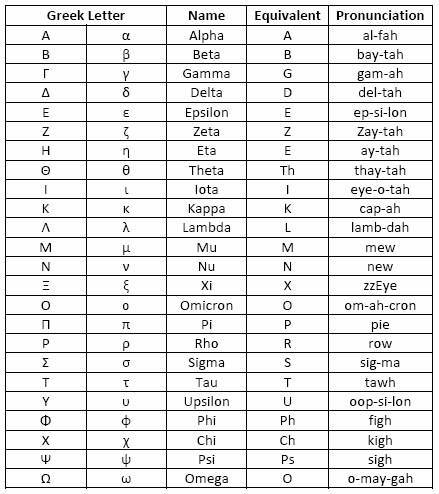
\includegraphics{apha.png}

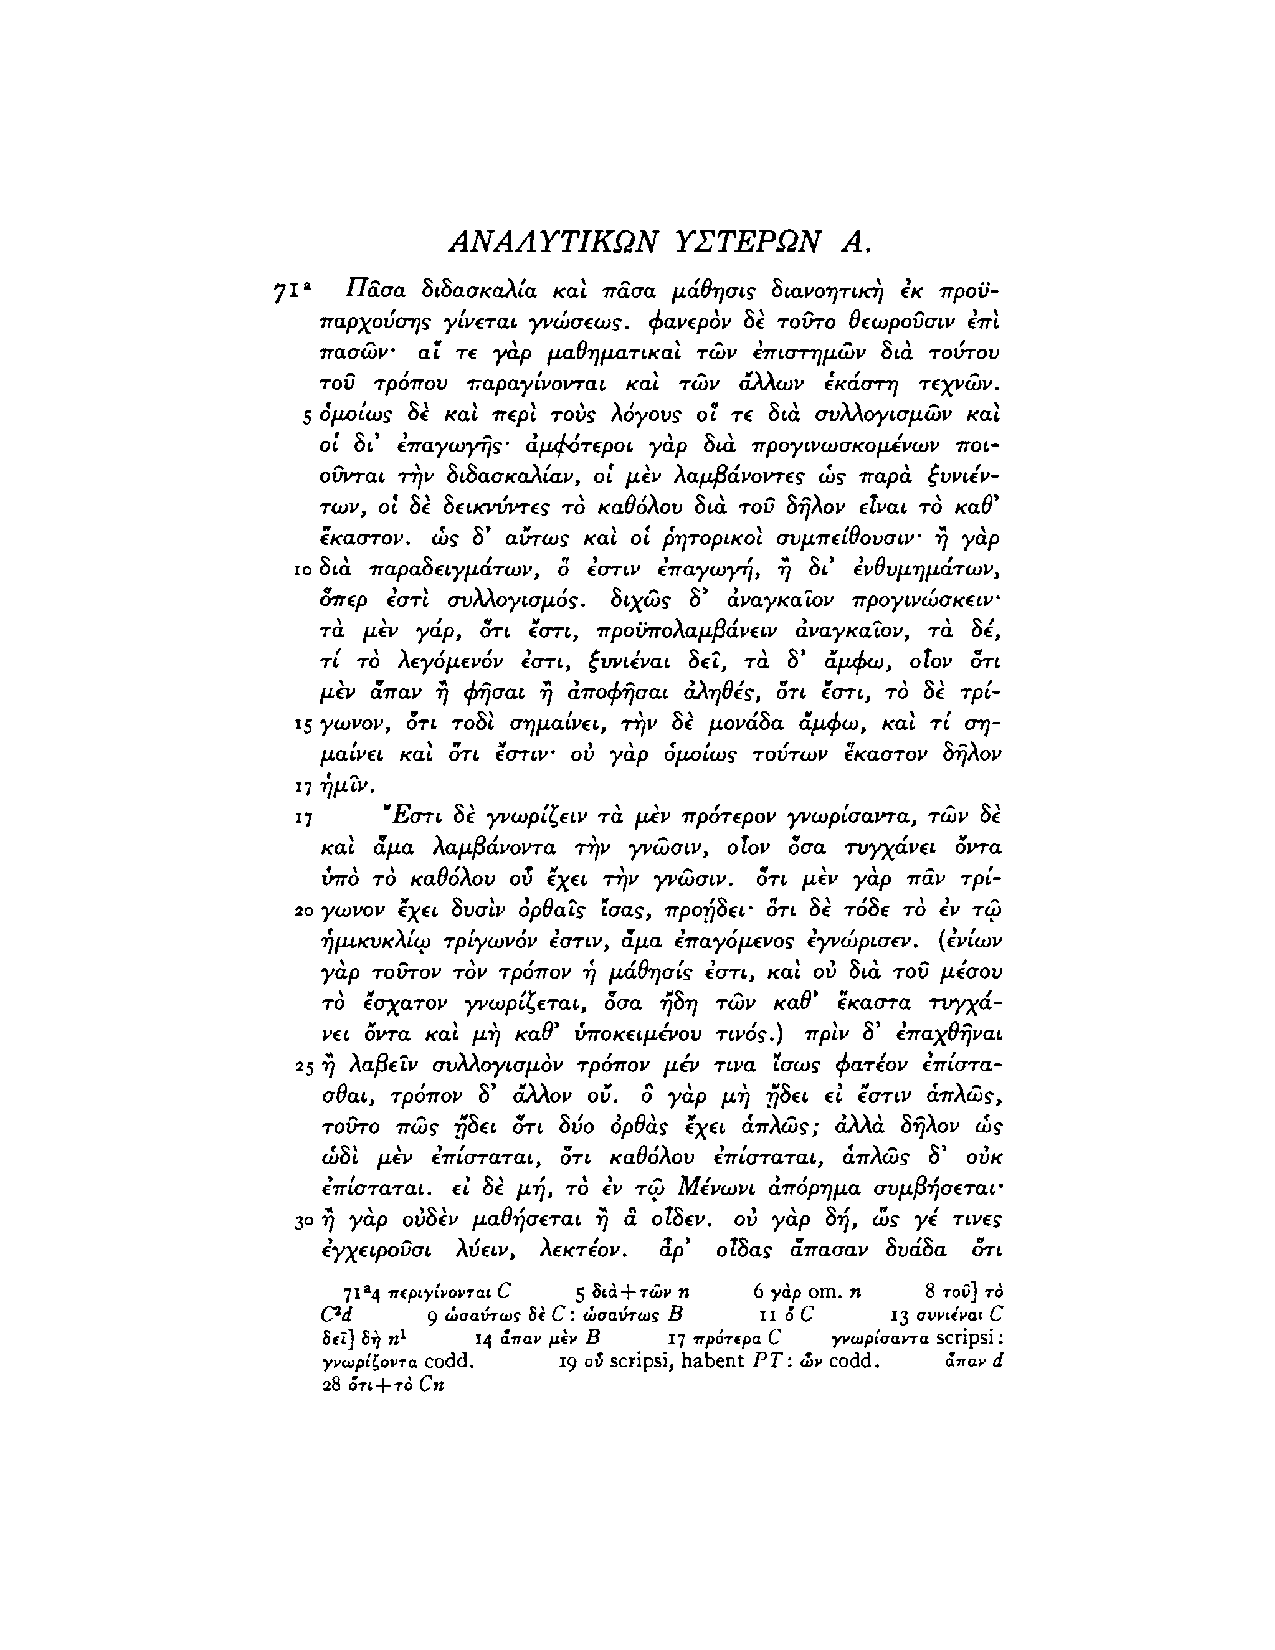
\includepdf{text.pdf}






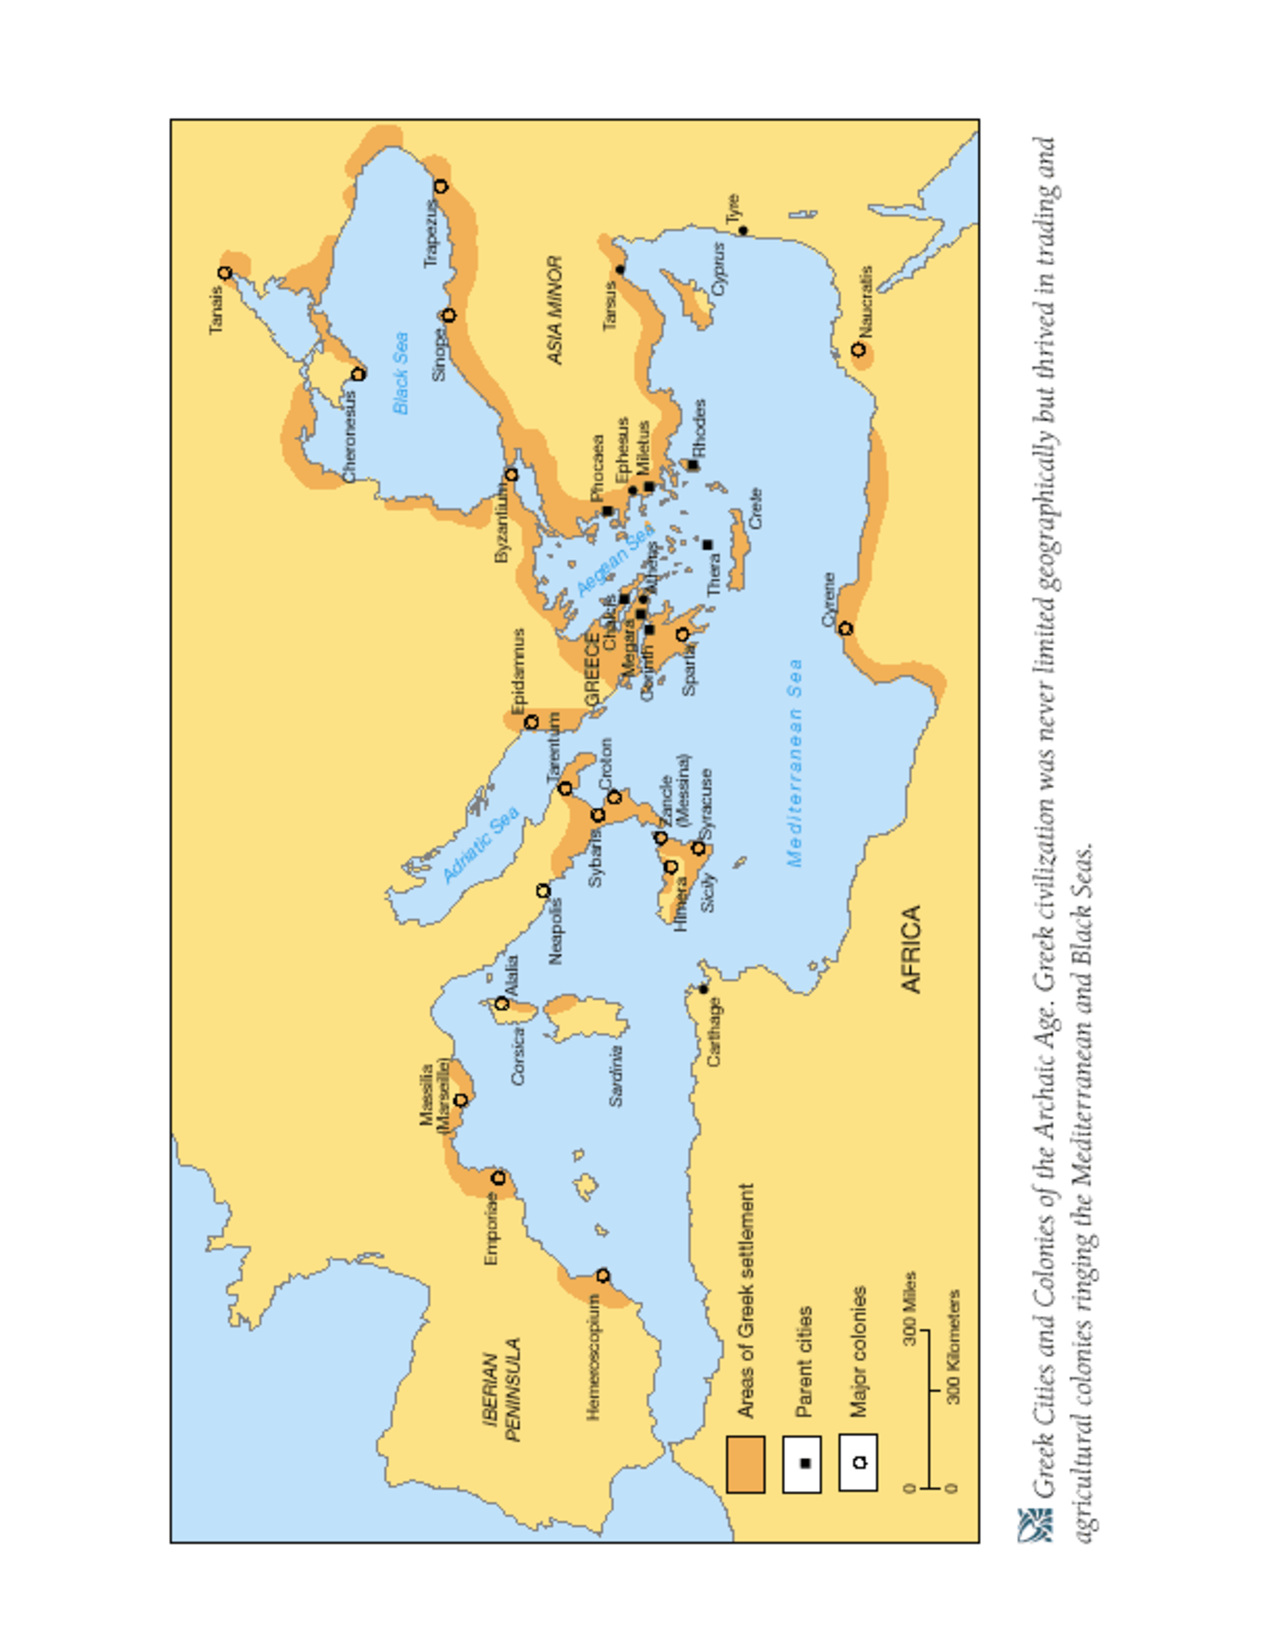
\includepdf{map.pdf}

\end{document}
